\section{Wirtschaftskrisen}
\subsection{Krise auf dem amerikanischen Immobilienmarkt 2006}
Nach 2001 verfolgte die USA eine sehr expansive Geldpolitik. Dadurch waren die Zinsen lange Zeit ungewöhnlich tief. Die tiefen Hypothekarzinsen verursachten ein rasches Ansteigen der Immobiliennachfrage und damit der Häuserpreise.\\
Gleichzeitig wurde ein innovatives Finanzinstrument kreiert – die ABS (asset-backed security). Damit konnten neu Tausende von einzelnen Hypotheken gebündelt und in handelbare Wertpapiere verwandelt werden (Verbriefung). Die ABS wurden, weil durch solide Immobilienfinanzierung gedeckt, als risikolos (Triple-A) eingeschätzt und rentierten besser als vergleichbare Anlagen wie z.B. Staatsanleihen.\\
Damit floss viel Kapital in den US-amerikanischen Immobiliensektor, die Häuserpreise stiegen unvermindert weiter und bildeten mit der Zeit eine eigentliche Finanzblase.\\
\textbf{Das $"$Subprime$"$-Segment}\\
Schwächen in der Regulierung des US-amerikanischen Immobilienmarktes führten dazu, dass zunehmend auch an finanzschwache Haushalte (Subprime-Segment) grosszügige Immobilienkredite ($"$Ninja-Kredite$"$ (NoIncomeNoJobNoAsset)) vergeben wurden.\\
Kreditgeber wie auch Kreditnehmer spekulierten auf zukünftige Wertsteigerungen der gekauften Immobilie. Mit diesen Wertsteigerungen sollten die anfallenden Zinszahlungen beglichen werden.\\
Mitte 2006 begannen die Häuserpreise in den USA landesweit drastisch zu sinken. Gründe dazu waren:
\begin{itemize}
	\item Ab 2004 hob die amerikanische Zentralbank schrittweise die Zinsen wieder an. Die Hypothekarzinsen der $"$Subprime$"$-Kredite stiegen dadurch rasch an.
	\item Die Immobiliennachfrage ging wegen den höheren Hypothekarzinsen zurück. Zudem mussten erste $"$Subprime$"$-Kreditnehmer ihre Immobilien an die Banken zurückgeben, weil sie die Zinsen nicht mehr bedienen konnten.
	\item Mit der zurückgehenden Nachfrage und dem steigenden Angebot nach Immobilien kamen die Häuserpreise rasch unter Druck. Die Banken reagierten mit einer vorsichtigeren Vergabe von Krediten (die Nachfragereduktion verstärkt sich dadurch).
	\item Die Preise der ABS sackten dadurch ins Bodenlose ab.
\end{itemize}
Der Preissturz der ABS hat für deren Käufer negative Folgen. Banken wie Bear Stearns oder BNP Paribas mussten erste $"$Subprime$"$-Fonds schliessen.\\
Dadurch wurde das Vertrauen der internationalen Banken untereinander erschüttert. Die Zinsen für Interbanken-Geschäfte (zur eigenen Liquiditätssicherung) erhöhten sich schlagartig, sofern überhaupt noch gegenseitig Kredite auf dem Geldmarkt gewährt wurden.
\begin{multicols}{3}
	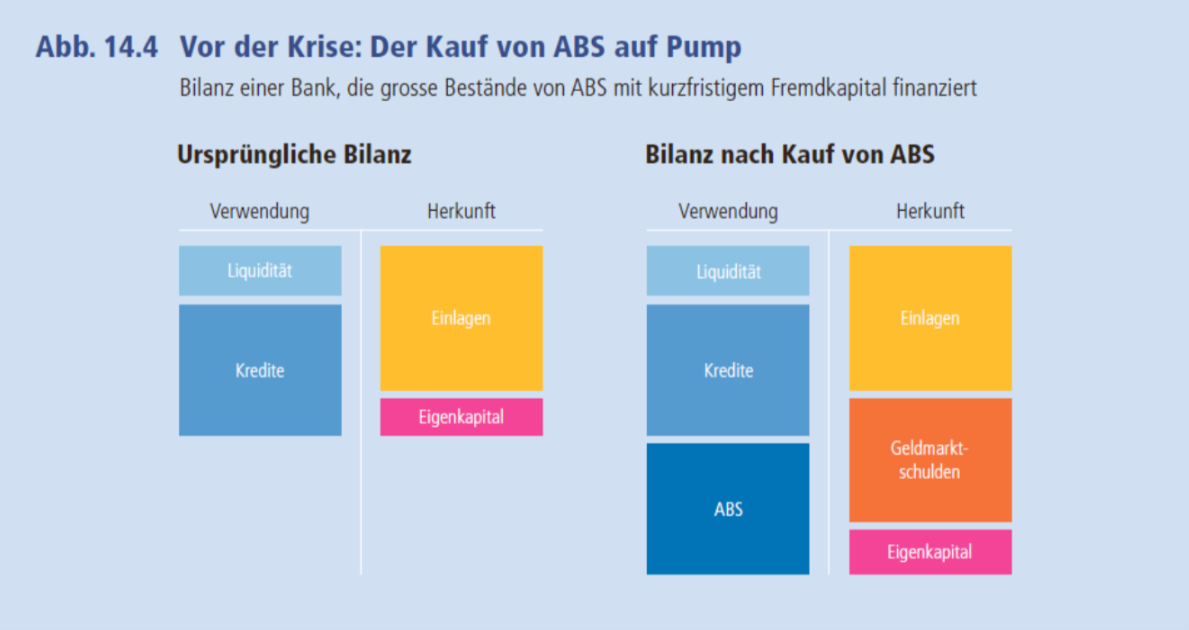
\includegraphics[width=\linewidth]{images/abs1.png}
	\columnbreak
	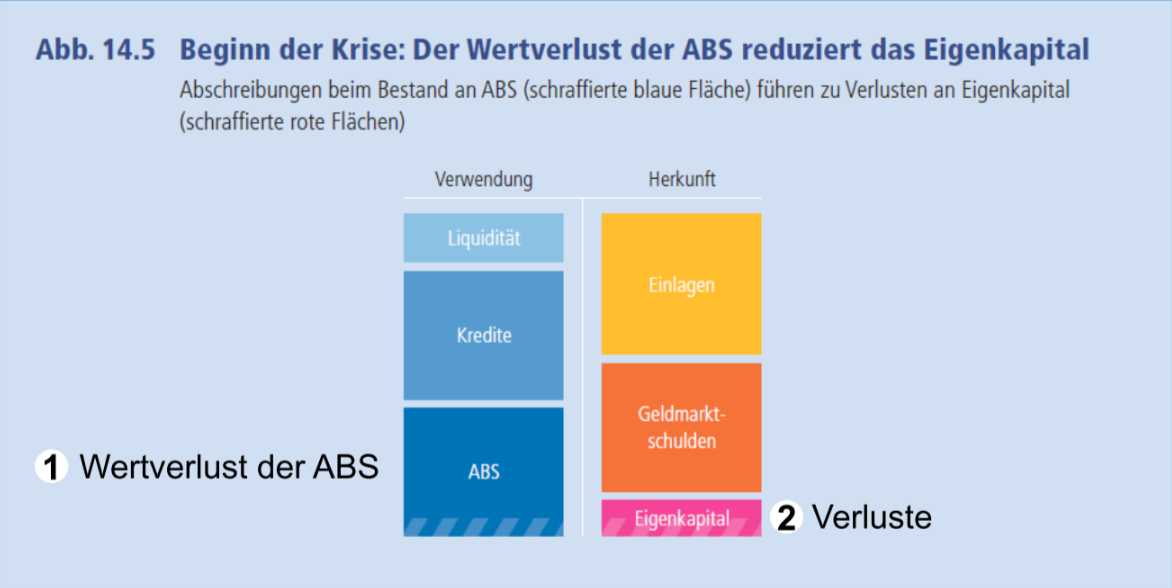
\includegraphics[width=\linewidth]{images/abs2.png}
	\columnbreak
	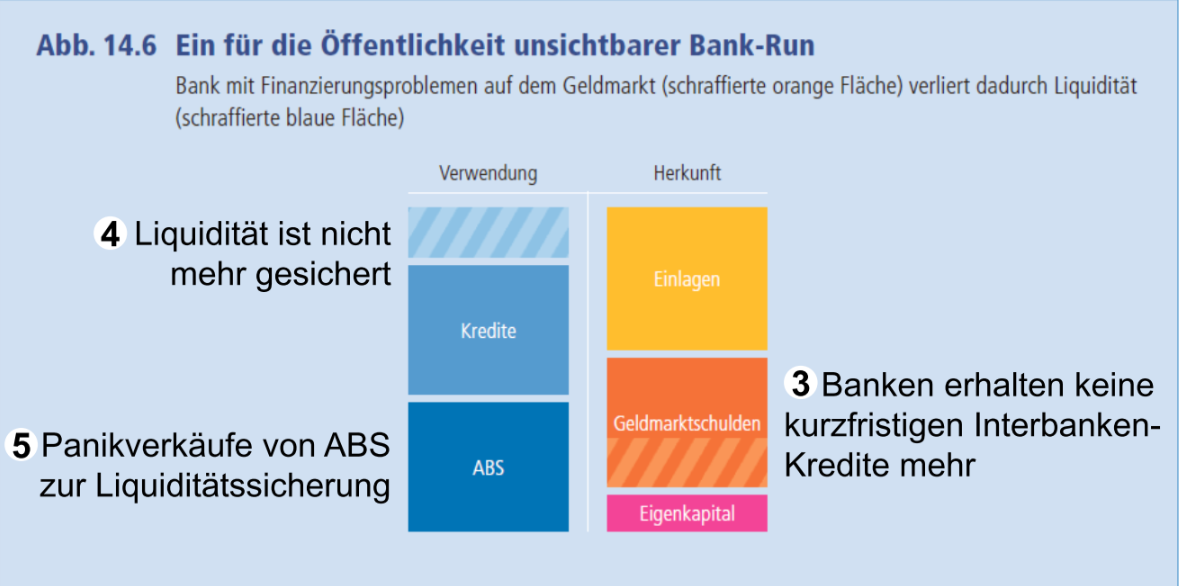
\includegraphics[width=\linewidth]{images/abs3.png}
\end{multicols}

\subsection{Euro-Krise von 2010 - auch eine Bankenkrise}
Die Einführung des Euro hat zum Aufbau von grossen makroökonomischen Ungleichgewichten geführt. Die Korrektur dieser Ungleichgewichte wäre zwangsläufig früher oder später erfolgt. Die aus der US-amerikanischen Immobilienkrise hervorgegangene weltweite Finanzkrise führte nun zu einem schockartigen Aufbrechen der Probleme der Euro-Zone.\\
Die Einführung des Euro bewirkte in den PIGS-Staaten
\begin{itemize}
	\item eine hohe Überschuldung (Zweifel an deren Rückzahlfähigkeit)
	\item einen Verlust an Wettbewerbsfähigkeit der Exportindustrie (durch zu hohe inländische Inflation).
\end{itemize}
Die weltweite aus den USA stammende Finanzkrise traf somit auf schon wirtschaftlich geschwächte Euro-Länder.\\
Die hoch verschuldeten Länder der Euro-Zone können ihre Schuldenproblematik nicht mehr selbst lösen. Üblicherweise bieten die Gläubiger in dieser Situation Hand zu einem Schuldennachlass bzw -umschuldung (z.B. zugunsten Entwicklungsländer).\\
Das Problem war nun, dass ein grosser Teil der Staatsanleihen von den Banken der europäischen Überschussländer gehalten wurden, welche aber durch die weltweite Finanzkrise schon unterkapitalisiert waren. Eine Umschuldung im grossen Stile hätte in diesen Banken zu existenziellen Problemen geführt.\\
Die weltweite Finanzkrise forderte die Banken in zwei Punkten:
\begin{itemize}
	\item Fehlende Liquidität, da das kurzfristige Interbankengeschäft wegen dem gegenseitigen Misstrauen unter den Banken teilweise zum Erliegen gekommen ist.
	\item Drohende Insolvenz, da die Verluste auf die Bestände von ABS und Staatspapieren die banküblich sehr knappe Eigenkapitaldeckung der Banken reduzierte.
\end{itemize}

\subsection{Die Rettung der UBS}
Im Herbst 2008 steht die UBS kurz vor dem Zusammenbruch. Finanzminister Hans-Rudolf Merz wird am 20. Sept. von Nationalbank und FINMA über die gravierende Lage der Bank informiert, erlebt aber selber wenige Tage später einen Herz-Kreislauf-Stillstand. Seine Stellvertreterin Eveline Widmer-Schlumpf muss das Finanzdepartement in diesen dramatischen Tagen interimistisch übernehmen. Am 15. Okt. beschliesst der Bundesrat ein sechs Milliarden Franken schweres Rettungspaket. Die Nationalbank übernimmt von der UBS faule Wertpapiere von max. 60 Milliarden Franken. Für ihr Krisenmanagement erhält Eveline Widmer-Schlumpf viel Lob.\\
Die UBS hatte über ihre US-amerikanische Tochtergesellschaft sehr stark in ABS investiert. Durch die Immobilienkrise in den USA fiel der Preis der ABS ins Bodenlose. Diese Verluste zehrten das Eigenkapital der UBS zunehmend auf.\\
2008 gelang es der UBS, zusätzliches Eigenkapital von asiatischen Investoren zu beschaffen. Dieses neue Kapital genügte aber nicht, um die ABS-Verluste zu kompensieren. Verunsicherte Kunden zogen darauf massiv Einlagen ab. Die UBS stand vor einem möglichen Kollaps.\\
Da die UBS eine der $"$Too Big to Fail$"$-Banken ist, entschlossen sich 2008 die schweizerischen Behörden (Bund und SNB) zu handeln.\\
Die staatliche Rettungsaktion sah wie folgt aus:
\begin{description}
	\item[Unterstützung auf der Passivseite:] Einschiessen von neuem Eigenkapital durch den Bund (6 Mia. Franken in Form eines Darlehens, welches er zu einem späteren Zeitpunkt in Aktien umwandeln konnte). 2009 verkaufte der Bund seine Aktien mit einem Gewinn von 1.2 Mia. Franken.
	\item[Unterstützung auf der Aktivseite:] Übernahme von 38.7 Mia. Franken an $"$vergifteten$"$ Wertpapieren durch die SNB und deren Überführung in eine neu gegründete $"$bad bank$"$. Die UBS musste 10\% dieser Summe für eine mögliche Verlustdeckung in diese $"$bad bank$"$ einschiessen. In etwa zwei Jahren dürften die letzten Wertpapiere verkauft sein. Ende 2013 hat die UBS definitiv den Stabilisierungsfond (bad bank) für 3.75 Mia. Franken von der SNB zurückgekauft.
\end{description}

\subsection{Der Fall Irland}
\textbf{Ursachen der Krise}\\
Der Beitritt zur Währungsunion liess die Zinsen sinken und ermöglichte es den Banken, den Markt mit billigen Immobilienkrediten zu fluten. Die verwandelten das Land in eine Grossbaustelle: Binnen weniger Jahre wuchs der Hausbestand um ein Drittel. Allein 2006 wurden im kleinen Irland 93000 Wohnungen fertig gestellt - 90\% mehr als noch zur Jahrtausendwende. Trotz des stark wachsenden Angebots an neuem Wohnraum stiegen die Häuserpreise immer weiter und schafften einen trügerischen Wohlstand. Die auf Pump finanzierte Nachfrage schien unersättlich. Auch Mittelklasse-Haushalte legten sich Zweit-, Dritt- und Viertimmobilien zu.\\
\textbf{Folgen der Krise}\\
Die irische Regierung hat die einheimischen Banken mit Hilfe in Milliardenhöhe vor dem Zusammenbruch gerettet. Die Institute hatten sich am Immobilienmarkt verspekuliert. Nach Schätzungen wird Irland für die Bankenrettung insgesamt etwa 50 Mia. Euro aufbringen müssen - bei einem BIP von 160 Mia. Euro. Das Haushaltsdefizit wird 2010 deshalb wohl 32\% der Wirtschaftsleistung ausmachen. Zusätzlich sind die Steuereinnahmen Irlands stark zurückgegangen.\\
\textbf{Monetarisierung der Staatsschulden}\\
Nachdem die irische Nationalbank nun mit einem abenteuerlichen Manöver den irischen Staat von Milliardenlasten befreit hat, steht zu befürchten, dass sich der Süden auch darin ein Vorbild nimmt und das Verbot monetärer Staatsfinanzierung für die Europäische Zentralbank das Papier nicht mehr wert ist, auf dem der Gesetzestext gedruckt ist.
